\documentclass[12pt, titlepage]{report}
\usepackage{consumer_resource_final}
\graphicspath{{./figures/}}

\begin{document}
\begin{figure}
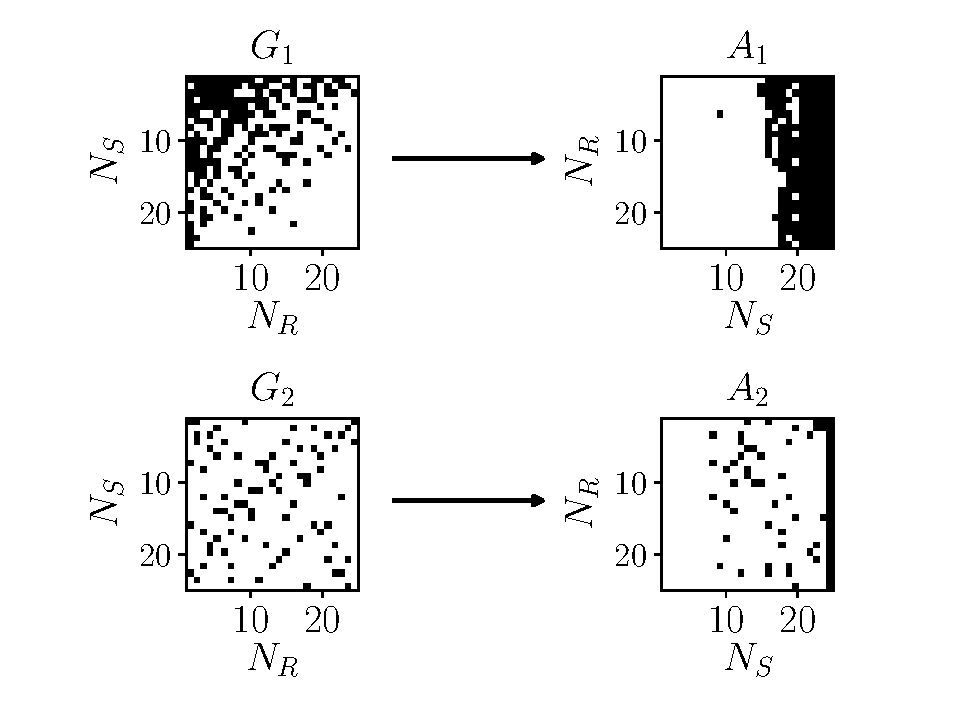
\includegraphics{typical_optimal_LRI_matrix}
\caption{Typical shape of the consumption $G_i$ and syntrophy $A_i$ matrices. The white cells symbolize a zero matrix element and the black cells, a one. $A_i$ here is the outcome of the LRI MC algorithm described in Methods \ref{section: methods LRI MC solver}. The first row has a consumption matrix with $\eta_1=0.6$ and $\kappa_1=0.32$, the LRI MC solver gives rise to a syntrophy matrix with same connectance and ecological overlap $\approx 0.85$. The second row has $G_2$ with $\eta_2=0.1$ and $\kappa_2=0.13$ and the corresponding syntrophy matrix $A_2$ has ecological overlap $\sim 0.42$. We observe that under this optimisation, species that consume few resources end up releasing many and the other way around.}\label{fig: dynamical stability results typical shape of consumption syntrophy LRI algorithm}
\end{figure}
\begin{figure}
  \begin{minipage}[c]{0.67\textwidth}
    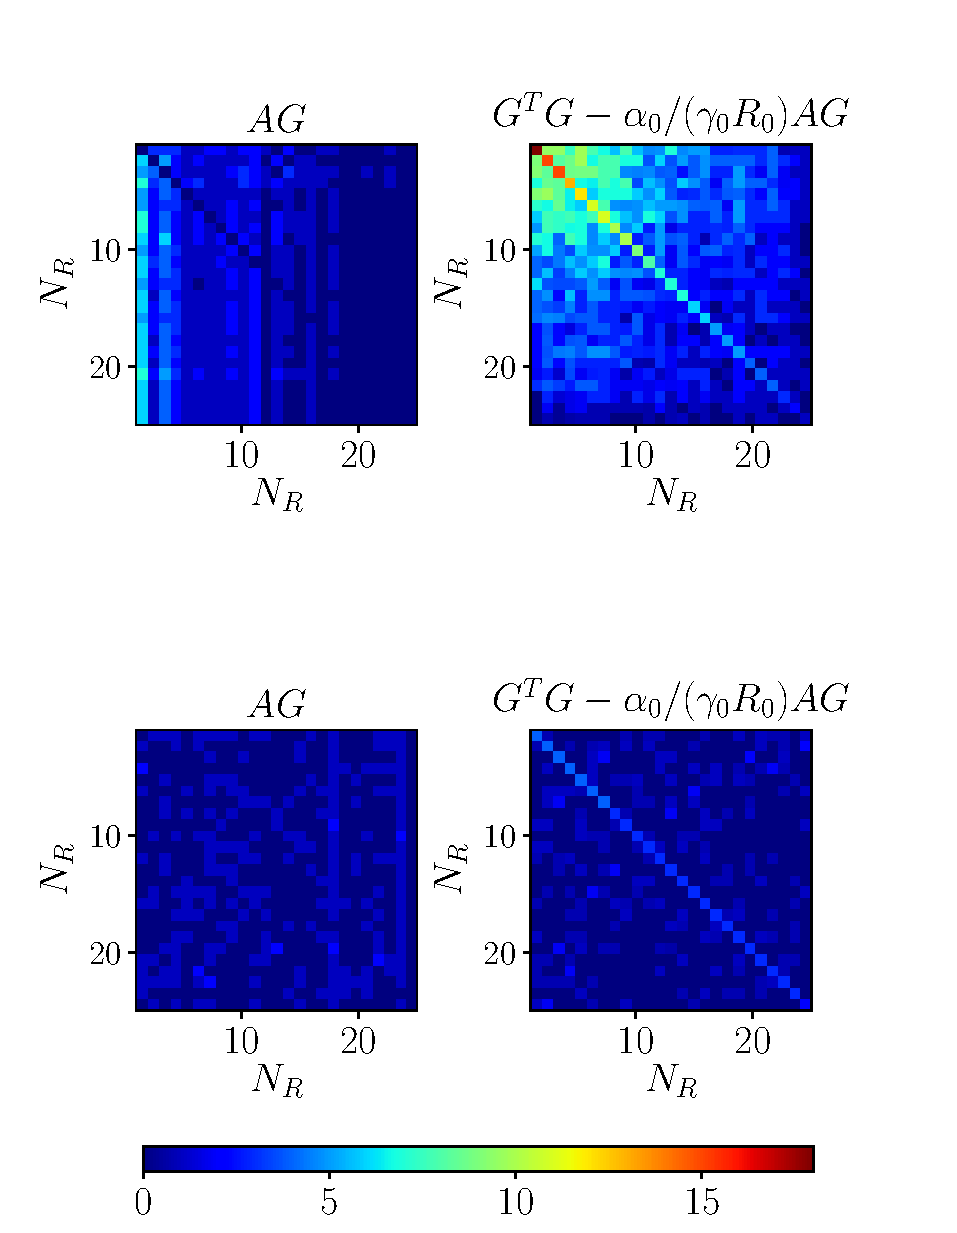
\includegraphics[width=\textwidth]{optimal_LRI_requirements}
  \end{minipage}\hfill
  \begin{minipage}[c]{0.3\textwidth}
    \caption{Plotting of $AG$ and $G^TG-\alpha_0/(\gamma_0R_0) AG$. The $A$ and $G$ matrices of the first and second rows correspond to the respective $A$ and $G$ of Figure \ref{fig: dynamical stability results typical shape of consumption syntrophy LRI algorithm}. As expected, we obtain an $A$ such that intraspecific coprophagy is limited (the diagonal of $AG$ is roughly zero) and, outside the diagonal, $G^TG-\alpha_0/(\gamma_0R_0) AG \approx 0$. Both relations are better satisfied for consumption (and hence syntrophy) matrices with a low connectance.}\label{fig: dynamical stability optimal LRI requirements met}
  \end{minipage}
\end{figure}
\begin{figure}
\captionsetup[subfigure]{captionskip = -180pt, margin = 42pt}
\hspace{-0.1\linewidth}
\subfloat[]{\includegraphics[width=0.6\linewidth]{{structure_alpha_matrix_NR25_NS25_with_nestedness}.pdf}}
\subfloat[]{\includegraphics[width=0.6\linewidth]{{structure_alpha_matrix_NR25_N25_with_connectance}.pdf}}

\hspace{-0.1\linewidth}
\subfloat[]{\includegraphics[width=0.6\linewidth]{{structure_alpha_matrix_NR50_NS25_with_nestedness}.pdf}}
\subfloat[]{\includegraphics[width=0.6\linewidth]{{structure_alpha_matrix_NR50_N25_with_connectance}.pdf}}
\caption{Properties of the syntrophy matrix against the consumption matrix. (a)-(c) Ecological overlap of $A$ as a function of the ecological overlap of $G$ for $N_S=25$ and $N_R=25$ (a) or $N_R=50$ (c). (b)-(d) Ecological overlap of $A$ as a function of the connectance of $G$ for $N_S=25$ and $N_R=25$ (b) or $N_R=50$ (d). The nestedness of the ``intraspecific syntrophy restricted'' is also plotted as a matter of comparison. As $\eta_G$ or $\kappa_G$ increase, the two results will without surprise give matrices with similar properties. \textbf{Explain this?}}
\label{fig: dynamical stability results nestedness LRI outcome}
\end{figure}
\begin{figure}
\captionsetup[subfigure]{captionskip=-225pt, margin=55pt}
\hspace{-0.1\linewidth}
\subfloat[]{\includegraphics[width=1.2\linewidth]{{probability_dynamical_stability_NR25_NS25_Nest0.5_Conn0.416_low_colorbar}.pdf}}

\vspace{-12pt}
\hspace{-0.1\linewidth}
\subfloat[]{\includegraphics[width=1.2\linewidth]{{probability_dynamical_stability_NR25_NS25_Nest0.5_Conn0.416_wo_title_high_colorbar}.pdf}}
\caption{Typical color plot local dynamical stability metaparameters function $\mathcal{D}_L$. for microbial communities with $\eta_G=0.5$ and $\kappa_G=0.42$. The color bar indicates the value of $\mathcal{D}_L\left((\gamma_0, S_0, \alpha_0), G, A\right)$ with $A$ fully connected. The plane is divided in two zones, one where $\mathcal{D}_L = 0$ and another where $\mathcal{D}_L\approx 1$ (the red and blue regions, respectively, in (a)). Upon further notice (b), it turns out the $\mathcal{D}_L \approx 1$ region is very patchy: we observe many $(\gamma_0, S_0, \alpha_0)$ configurations for which $\mathcal{D}_L$ is very close but not exactly equal to $1$. These points are \textit{almost} fully dynamically stable.} \label{fig : dynamical stability results typical dynamical stability function}
\end{figure}
\begin{figure}
\vspace{-84pt}
\hspace{-0.1\linewidth}
\includegraphics[width=1.2\linewidth]{{common_dynamical_stability_region_NR25_NS25}.pdf}
\caption{Common full local dynamical stability volume for different $A$ structures: (a) fully connected, (b) no intraspecific syntrophy and (c) LRI algorithm. The points coloured in dark red give rise to locally dynamically stable systems with probability 1 for \important{all the matrices considered}. Very few spots verify this property when there is no syntrophic interaction, and no point gives rise to a fully dynamically stable system for $\alpha_0 = \num{1.3e-3}$. This is independent of the structure of $A$ that we chose. The white points never give rise to fully dynamically stable systems.}\label{fig: dynamical stability results common fully dynamically stable volume}
\end{figure}
\begin{figure}
\captionsetup[subfigure]{captionskip = -180pt, margin = 52pt}
%\vspace{-96pt}
\hspace{-0.15\linewidth}
\subfloat[\label{fig: lds region results Nest 0.35 Conn 0.2208}]{\includegraphics[width=1.3\linewidth]{{local_dynamical_stability_wt_wc_region_NR25_NS25_Nest0.35_Conn0.2208}.pdf}}

\vspace{-44pt}
\hspace{-0.15\linewidth}
\subfloat[]{\includegraphics[width=1.3\linewidth]{{local_dynamical_stability_wt_wc_region_NR25_NS25_Nest0.35_Conn0.3216}.pdf}}

\vspace{-44pt}
\hspace{-0.15\linewidth}
\subfloat[\label{fig: lds region results Nest 0.35 Conn 0.272}]{\includegraphics[width=1.3\linewidth]{{local_dynamical_stability_wt_region_NR25_NS25_Nest0.35_Conn0.272}.pdf}}

\caption{Locally fully dynamically stable region $\mathcal{D}_{L,1}^{G,A}$ as a function of syntrophy for different matrices $G$. The white zone corresponds to points that are never fully locally dynamically stable. The colour of a given point tells until which syntrophy that point is fully locally dynamically stable, \eg
a green point is fully locally dynamically stable for $0 \leq \alpha_0 \leq \num{6.5e-3}$. Row (a) corresponds to $G$ with $\eta_G = 0.35$ and $\kappa_G = 0.23$, (b) has $\eta_G=0.35$ and $\kappa_G=0.33$ and (c) $\eta_G=0.35$ and $\kappa_G=0.27$. Even at fixed ecological overlap, different connectances of $G$ give rise to completely different systems in terms of local dynamical stability.}\label{fig: dynamical stability results local dynamical stability region for different matrices}
\end{figure}

\begin{figure}
\captionsetup[subfigure]{captionskip=-210pt, margin=28pt}
\hspace{-0.1\linewidth}
\subfloat[]{\includegraphics[width=0.6\linewidth]{{local_dynamical_stability_average_gamma0}.pdf}}
\subfloat[]{\includegraphics[width=0.6\linewidth]{{local_dynamical_stability_average_S0}.pdf}}
\caption{(a) Average consumption rate $\av{\gamma_0}_D(\alpha_0)$ and (b) average resource abundance equilibrium
$\av{S_0}_D(\alpha_0)$ as a function of syntrophy (a formal definition of $(\av{\gamma_0}_D(\alpha_0), \av{S_0}_D(\alpha_0))$ is provided in Appendix \ref{app : center of gravity local dynamical stability}). Intuitively, $(\av{\gamma_0}_D(\alpha_0), \av{S_0}_D(\alpha_0))$ represents the center $(\gamma_0,S_0)$ point of $\mathcal{D}^{G,A}_{L,1}\left(\alpha_0\right)$,  averaged over all matrices $(G,A) \in S_{25}$, or as we call it the ``\important{center of dynamical stability}''. As syntrophy increases, only points with a large consumption rate and a small resource abundance at equilibrium remain dynamically stable. The sudden drop of $\av{\gamma_0}_D$ (and rise of $\av{S_0}_D$) at $\alpha_0=\num{9.1e-3}$ is a finite-size effect. Indeed we only monitor points in the unit square $[0,1]^2$, such that the $(G,A)$ for which the center of $\mathcal{D}_{L,1}^{G,A}(\alpha_0)$ leave that zone at $\alpha_0=\num{9.1e-3}$ do not contribute to $(\av{\gamma_0}_D, \av{S_0}_D)$ anymore. Only the $(G,A)$ which previously had a lower, resp. higher, contribution to $\av{\gamma_0}_D$, resp. $\av{S_0}_D$, are taken into account, which results in that strange behaviour. The fact that $\av{\gamma_0}_D$ continues to increase (and $\av{S_0}_D$ to decrease) after that point show that this reasoning is right.}\label{fig : dynamical stability results center of stability}
\end{figure}

% \begin{figure}
% \captionsetup[subfigure]{captionskip = -230pt, margin = 50pt}
% \vspace{-96pt}
% \hspace{-0.1\linewidth}
% \subfloat[]{\includegraphics[width=1.2\linewidth]{{feasibility_vs_lds_NR25_NS25_Nest0.1_Conn0.1296}.pdf}}
%
% \hspace{-0.1\linewidth}
% \subfloat[]{\includegraphics[width=1.2\linewidth]{{feasibility_vs_lds_NR25_NS25_Nest0.6_Conn0.3168}.pdf}}
%
% \caption{Ratio of the size of the fully dynamically stable volume and the fully feasible volume for two consumption matrices $G$ (a) with $\eta_G=0.1$ and $\kappa_G=0.13$, (b) with $\eta_G=0.6$ and $\kappa_G=0.32$. We observe different behaviours for different matrices: for (a) feasibility does not imply local dynamical stability even without syntrophy (it is barely feasible but the ratio is a bit below one for $\alpha_0=0$). On the other hand, for (b) feasibility implies local dynamical stability, indeed both regions have the same volume and since $\mathcal{D}_{L,1}^{G,A}(\alpha_0) \subset \mathcal{F}^{G,A}_1(\alpha_0)$, we conclude that both are equal.}
% \end{figure}
\begin{figure}
%\captionsetup[subfigure]{captionskip=-10}
\hspace{-0.1\linewidth}
\captionsetup[subfigure]{captionskip=-140pt}
\subfloat[]{\includegraphics[width=0.4\linewidth]{{prob_dyn_stab_if_feas_NR25.0_NS25.0_Nest0.5_Conn0.416}.pdf}}
\subfloat[]{\includegraphics[width=0.4\linewidth]{{prob_dyn_stab_if_feas_NR25.0_NS25.0_Nest0.45_Conn0.384}.pdf}}
\subfloat[]{\includegraphics[width=0.4\linewidth]{{prob_dyn_stab_if_feas_NR25.0_NS25.0_Nest0.2_Conn0.0896}.pdf}}

\caption{Plot of the probability that a microbial community is dynamically stable under the assumption that it is feasible for different consumption-syntrophy networks $(G,A)$. The different lines on the same subplot show the four different $A$-scenarios. The results differ with the consumption matrix considered: (a) $\eta_G=0.5$, $\kappa_G=0.43$, (b) $\eta_G=0.45$, $\kappa_G=0.38$ and (c) $\eta_G=0.2$, $\kappa_G=0.08$. }
\label{fig : dynamical stability results proba feas -> dyn sta}
\end{figure}

\begin{figure}
\hspace{-0.1\linewidth}
\captionsetup[subfigure]{captionskip=-205pt, margin=55pt}
\subfloat[]{\includegraphics[width=0.6\linewidth]{{size_local_dynamical_stability_region_NR25_NS25_Nest0.3_Conn0.2816}.pdf}}
\subfloat[]{\includegraphics[width=0.6\linewidth]{{size_local_dynamical_stability_region_NR25_NS25_Nest0.5_Conn0.416}.pdf}}

\caption{Evolution of the dynamically stable volume $\text{Vol}\left(\mathcal{D}_{L,1}^{G,A}\left(\alpha_0\right)\right)$ (see Appendix \ref{app: how to measure volume}) with $\alpha_0$ for different $(G,A) \in S_{25}$. (a) $\eta_G=0.3$ and $\kappa_G=0.28$, (b) $\eta_G=0.5$ and $\kappa_G=0.43$. The cross-shaped points indicate the data as measured numerically while the solid lines are the corresponding exponential fit (see main text). The four colors indicate the four $A$-scenarios considered. Independent of the $(G,A)$ network, fewer points are dynamically stable as syntrophy increases.}
\label{fig: dynamical stability results typical shrinkage of dynamical volume}
\end{figure}
% \begin{figure}
% \captionsetup[subfigure]{captionskip = -185pt, margin = 52pt}
% \vspace{-84pt}
% \hspace{-0.1\linewidth}
% \subfloat[]{\includegraphics[width=0.6\linewidth]{{largest_eigenvalue_NR25_NS25_critical_alpha0_fixed_connectance_random_structure}.pdf}}
% \subfloat[]{\includegraphics[width=0.6\linewidth]{{largest_eigenvalue_NR25_NS25_critical_alpha0_fixed_nestedness_random_structure}.pdf}}
%
% \vspace{-12pt}
% \hspace{-0.1\linewidth}
% \subfloat[]{\includegraphics[width=0.6\linewidth]{{largest_eigenvalue_NR25_NS25_critical_alpha0_fixed_connectance_no_release_when_eat}.pdf}}
% \subfloat[]{\includegraphics[width=0.6\linewidth]{{largest_eigenvalue_NR25_NS25_critical_alpha0_fixed_nestedness_no_release_when_eat}.pdf}}
%
% \vspace{-12pt}
% \hspace{-0.1\linewidth}
% \subfloat[]{\includegraphics[width=0.6\linewidth]{{largest_eigenvalue_NR25_NS25_critical_alpha0_fixed_connectance_optimal_matrix}.pdf}}
% \subfloat[]{\includegraphics[width=0.6\linewidth]{{largest_eigenvalue_NR25_NS25_critical_alpha0_fixed_nestedness_optimal_matrix}.pdf}}
% \vspace{-12pt}
% \caption{Critical syntrophy $\alpha_0^D$, defined as the smallest syntrophy for which we can still find metaparameters that will give rise to fully dynamically stable systems. How $\alpha_0^D$ is estimated is explained in the main text. Errors on $\alpha_0^D$ are not plotted but are at most around $10\%$. (a)(c)(e) Evolution of $\alpha_0^D$ with ecological overlap $\eta$ at different connectance. (b)(d)(f) Evolution of $\alpha_0^D$ with connectance $\kappa$ for different ecological overlap. We observe a strong trend: for a given connectance, $\alpha_0^D$ decreases as ecological overlap increases. Also, for a given ecological overlap, $\alpha_0^D$ increases as connectance is increased.}\label{fig: dynamical stability results critical dynamical syntrophy}
% \end{figure}
\begin{figure}
\vspace{-60pt}
\hspace{-0.1\linewidth}
\captionsetup[subfigure]{captionskip=-202pt, margin=42pt}
\subfloat[]{\includegraphics[width=0.6\linewidth]{{local_dynamical_stability_NR25_NS25_dyn_stability_decay_rate_fixed_nestedness_fully_connected}.pdf}}
\subfloat[]{\includegraphics[width=0.6\linewidth]{{local_dynamical_stability_NR25_NS25_dyn_stability_decay_rate_fixed_connectance_fully_connected}.pdf}}
\caption{Dynamical stability decay rate $d_D(G,A)$ for the $A$-matrix fully connected (FC scenario) and every $G \in G_{25}$, (a) as a function of connectance $\kappa_G$ for fixed ecological overlap $\eta_G$ and (b) as a function of ecological overlap for fixed connectance. The trend confirms the previous observations: at fixed ecological overlap, a microbial community with a more connected consumption matrix will sustain a larger syntrophy (\ie have a smaller decay rate) and at fixed connectance, systems with a small ecological overlap remain dynamically stable as syntrophy grows.}\label{fig: dynamical stability results dynamical decay rate FC}
\end{figure}

\begin{figure}
\vspace{-35pt}
\captionsetup[subfigure]{captionskip = -188pt, margin = 45pt}
\hspace{-0.05\linewidth}
\subfloat[]{\includegraphics[width=0.55\linewidth]{{local_dynamical_stability_NR25_NS25_dyn_stability_decay_rate_away_from_FC_fixed_nestedness_no_release_when_eat}.pdf}}
\subfloat[]{\includegraphics[width=0.55\linewidth]{{local_dynamical_stability_NR25_NS25_dyn_stability_decay_rate_away_from_FC_syntrophy_fixed_connectance_no_release_when_eat}.pdf}}

\vspace{-12pt}
\hspace{-0.05\linewidth}
\subfloat[]{\includegraphics[width=0.55\linewidth]{{local_dynamical_stability_NR25_NS25_dyn_stability_decay_rate_away_from_FC_fixed_nestedness_optimal_matrix}.pdf}}
\subfloat[]{\includegraphics[width=0.55\linewidth]{{local_dynamical_stability_NR25_NS25_dyn_stability_decay_rate_away_from_FC_syntrophy_fixed_connectance_optimal_matrix}.pdf}}

\vspace{-12pt}
\hspace{-0.05\linewidth}
\subfloat[]{\includegraphics[width=0.55\linewidth]{{local_dynamical_stability_NR25_NS25_dyn_stability_decay_rate_away_from_FC_fixed_nestedness_random_structure}.pdf}}
\subfloat[]{\includegraphics[width=0.55\linewidth]{{local_dynamical_stability_NR25_NS25_dyn_stability_decay_rate_away_from_FC_syntrophy_fixed_connectance_random_structure}.pdf}}

\vspace{-12pt}
\caption{Relative deviation away from the $FC$ case dynamical stability decay rate as a function of the characteristics of the consumption matrix $G$. A positive $y$-coordinate means that the considered scenario provides a $d_D(G,A)$ smaller than the $FC$ case and is in consequence a sign that the network can better withstand an increase in syntrophy while remaining dynamically stable. We considered the three usual scenarios for the $A$-matrix: (a)-(b) NIS, (c)-(d) LRI and (e)-(f) RS. \textbf{TO DO: compute errors on this graph}}\label{fig : dynamical stability results decay rate away from FC case}
\end{figure}

% \begin{figure}
% \captionsetup[subfigure]{captionskip = -185pt, margin = 52pt}
% \vspace{-84pt}
% \hspace{-0.1\linewidth}
% \subfloat[]{\includegraphics[width=0.6\linewidth]{{largest_eigenvalue_NR25_NS25_critical_alpha0_fixed_connectance_random_structure}.pdf}}
% \subfloat[]{\includegraphics[width=0.6\linewidth]{{largest_eigenvalue_NR25_NS25_critical_alpha0_fixed_nestedness_random_structure}.pdf}}
%
% \vspace{-12pt}
% \hspace{-0.1\linewidth}
% \subfloat[]{\includegraphics[width=0.6\linewidth]{{largest_eigenvalue_NR25_NS25_critical_alpha0_fixed_connectance_no_release_when_eat}.pdf}}
% \subfloat[]{\includegraphics[width=0.6\linewidth]{{largest_eigenvalue_NR25_NS25_critical_alpha0_fixed_nestedness_no_release_when_eat}.pdf}}
%
% \vspace{-12pt}
% \hspace{-0.1\linewidth}
% \subfloat[]{\includegraphics[width=0.6\linewidth]{{largest_eigenvalue_NR25_NS25_critical_alpha0_fixed_connectance_optimal_matrix}.pdf}}
% \subfloat[]{\includegraphics[width=0.6\linewidth]{{largest_eigenvalue_NR25_NS25_critical_alpha0_fixed_nestedness_optimal_matrix}.pdf}}
% \vspace{-12pt}
% \caption{Critical syntrophy $\alpha_0^D$, defined as the smallest syntrophy for which we can still find metaparameters that will give rise to fully dynamically stable systems. How $\alpha_0^D$ is estimated is explained in the main text. Errors on $\alpha_0^D$ are not plotted but are at most around $10\%$. (a)(c)(e) Evolution of $\alpha_0^D$ with ecological overlap $\eta$ at different connectance. (b)(d)(f) Evolution of $\alpha_0^D$ with connectance $\kappa$ for different ecological overlap. We observe a strong trend: for a given connectance, $\alpha_0^D$ decreases as ecological overlap increases. Also, for a given ecological overlap, $\alpha_0^D$ increases as connectance is increased.}\label{fig: dynamical stability results critical dynamical syntrophy}
% \end{figure}



\begin{figure}
\vspace{-40pt}
\captionsetup[subfigure]{margin=40pt}
\hspace{-0.1\linewidth}
\subfloat[]{\includegraphics[width=1.2\linewidth]{{largest_eigenvalue_wt_NR25_NS25_Nest0.1_Conn0.1296_alpha0=0.0}.pdf}}

\vspace{-12pt}
\hspace{-0.1\linewidth}
\subfloat[]{\includegraphics[width=1.2\linewidth]{{largest_eigenvalue_wt_NR25_NS25_Nest0.1_Conn0.1296_alpha0=0.0039}.pdf}}

\vspace{-12pt}
\hspace{-0.1\linewidth}
\subfloat[]{\includegraphics[width=1.2\linewidth]{{largest_eigenvalue_wt_NR25_NS25_Nest0.1_Conn0.1296_alpha0=0.0078}.pdf}}
\caption{Largest real eigenvalue $\text{Re}(\lambda_1)$ averaged over 300 \textbf{TO DO : check number} realisations for each $(\gamma_0, S_0)$ points for the consumption matrix $G$ with consumers overlap $\eta_G = 0.1$ and connectance $\kappa_G=0.13$. The white points correspond to not fully dynamically stable systems. Each row corresponds to a different syntrophy value (a) $\alpha_0 = 0$ (no syntrophic interaction), (b) $\alpha_0 = \num{3.9e-3}$ and (c) $\alpha_0 = \num{7.8e-3}$. The different columns correspond to the different $A$ scenarios considered, which change the shape of the dynamically stable region as seen in the main text. As expected, the boundary points close to the $\gamma_0 \sim S_0^{-1}$ curve are the most stable in every situation. Points with a large $\gamma_0$ are the most stable of the unit square. }\label{fig: local dynamical stability results largest eigenvalue}
\end{figure}

\begin{figure}
\hspace{-0.1\linewidth}
\captionsetup[subfigure]{captionskip = -210pt, margin = 26pt}
\subfloat[\label{fig: dynamical stability results typical maximal eigenvalue observed varying syntrophy}]{\includegraphics[width=0.6\linewidth]{{largest_eigenvalue_varying_syntrophy_NR25_NS25_Nest0.3_Conn0.2272}.pdf}}
\subfloat[\label{fig: dynamical stability results shrinkage of DL1G varying syntrophy}]{\includegraphics[width=0.6\linewidth]{{size_local_dynamical_stability_region_NR25_NS25_Nest0.3_Conn0.2272}.pdf}}
\caption{For a consumption matrix $G$ with $\eta_G=0.3$ and $\kappa_G=0.23$. (a) Evolution of the maximal $\abs{\av{\real{\lambda_1}}}$ observed in the $(\gamma_0,S_0) \in [0,1]^2$ region. The maximal eigenvalue increases in magnitude, making the system more dynamically stable, as syntrophy increases. That trend is true for all matrices we considered. (b) Volume of $\mathcal{D}^G_{L,1}(\alpha_0)$. As syntrophy increases, fewer and fewer points become fully dynamically stable. For both figures, the different lines show the different stand for the different structure of the syntrophy matrix that we considered. \textbf{TO DO: replace this with average version}}\label{fig: results dynamical stability maximum eigenvalue observed vs size of dynamical region 25x25}
\end{figure}

\begin{figure}
\hspace{-0.15\linewidth}
\subfloat[]{\includegraphics[width=1.3\linewidth]{{local_dynamical_stability_region_NR25_NS25_Nest0.45_Conn0.3168}.pdf}}

\subfloat[]{\includegraphics[width=\linewidth]{{local_dynamical_stability_region_NR50_NS25_Nest0.45_Conn0.3328}.pdf}}
\caption{Fully dynamically stable region $\mathcal{D}^{G,A}_{L,1}$ with the three different structures of $A$ considered: fully connected (left), no intraspecific syntrophy (middle) and LRI matrix (right). The two matrices have the same ecological overlap and connectance, only the number of resources changes. (a) $G$ has $N_R=25$, $N_S=25$ and $\kappa_G=0.32$ and $\eta_G=0.45$. (b) $G$ has $N_R=50$, $N_S=25$ and $\kappa_G=0.33$ and $\eta_G=0.45$ (by lack of time, a fewer resolution on the unit square had to be taken). At $NR=50$, the fully dynamically stable region seems less fractured. The fact that more points can sustain an increased syntrophy is a trend for most of the matrices of the set. \textbf{still check this: the others are more less the same or a tad less}.} \label{fig: dynamical stability results typical lds region NR=50 NS=25}
\end{figure}
\begin{figure}
\hspace{-0.1\linewidth}
\captionsetup[subfigure]{captionskip = -210pt, margin = 26pt}
\subfloat[\label{fig: dynamical stability results typical maximal eigenvalue observed varying syntrophy NR=50}]{\includegraphics[width=0.6\linewidth]{{largest_eigenvalue_varying_syntrophy_NR50_NS25_Nest0.3_Conn0.2296}.pdf}}
\subfloat[\label{fig: dynamical stability results shrinkage of DL1G varying syntrophy NR=50}]{\includegraphics[width=0.6\linewidth]{{size_local_dynamical_stability_region_NR50_NS25_Nest0.3_Conn0.2296}.pdf}}
\caption{To be compared with Fig.\ref{fig: results dynamical stability maximum eigenvalue observed vs size of dynamical region 25x25}. The consumption matrix $G$ considered here has $\eta_G=0.3$ and $\kappa_G=0.23$. (a) Maximal average $\abs{\real{\lambda_1}}$ observed in the unit square. (b) Percentage of the unit square occupied by the fully dynamically stable region of $G$ as a function of syntrophy. The matrix considered has almost equal properties to the one in Fig.\ref{fig: results dynamical stability maximum eigenvalue observed vs size of dynamical region 25x25}, with the only difference that $N_R=50$ here. Even though the size of $\mathcal{D}_{L,1}^{G,A}$ is smaller, the eigenvalues are larger in magnitude.}
\end{figure}

% \begin{figure}
% \vspace{-72pt}
% \hspace{-0.0\linewidth}
% \subfloat[]{\includegraphics[width=\linewidth]{{largest_eigenvalue_wt_NR50_NS25_Nest0.1_Conn0.0832_alpha0=0.0}.pdf}}
%
% \vspace{-26pt}
% \hspace{-0.0\linewidth}
% \subfloat[]{\includegraphics[width=\linewidth]{{largest_eigenvalue_wt_NR50_NS25_Nest0.1_Conn0.0832_alpha0=0.0013}.pdf}}
%
% \vspace{-26pt}
% \hspace{-0.0\linewidth}
% \subfloat[]{\includegraphics[width=\linewidth]{{largest_eigenvalue_wt_NR50_NS25_Nest0.1_Conn0.0832_alpha0=0.0039}.pdf}}
% \caption{To be compared with \ref{fig: local dynamical stability results largest eigenvalue} \textbf{Is it really fair? No comparison because connectance is overall quite different and we saw that changing connectance can have quite a dramatic effect}, the zone is smaller but more stable (by a lot) can we really say this?.}\label{fig: dynamical stability results largest eigenvalue NR=50 NS=25}
% \end{figure}

\begin{figure}
\vspace{-84pt}
\hspace{-0.1\linewidth}
\subfloat[]{\includegraphics[width=0.6\linewidth]{{common_local_dynamical_stability_volume_NR50_NS25_varying_syntrophy_random_structure}.pdf}}
\subfloat[]{\includegraphics[width=0.6\linewidth]{{common_local_dynamical_stability_volume_NR50_NS25_varying_syntrophy_no_release_when_eat}.pdf}}

\centering
\subfloat[]{\includegraphics[width=0.6\linewidth]{{common_local_dynamical_stability_volume_NR50_NS25_varying_syntrophy_optimal_matrix}.pdf}}
\caption{Common fully dynamically stable volume. It is larger with a larger number of resources -> even though individually it is not always better, it is better for the worse matrices (since the common volume can handle more syntrophy)}\label{fig: dynamical stability results common lds volume NR=50 NS=25}
\end{figure}

\begin{figure}
\vspace{-84pt}
\captionsetup[subfigure]{captionskip=-202pt, margin=45pt}
\hspace{-0.1\linewidth}
\subfloat[]{\includegraphics[width=0.6\linewidth]{{local_dynamical_stability_decay_rate_50_vs_25_fixed_connectance_fully_connected}.pdf}}
\subfloat[]{\includegraphics[width=0.6\linewidth]{{local_dynamical_stability_decay_rate_50_vs_25_fixed_nestedness_fully_connected}.pdf}}

\hspace{-0.1\linewidth}
\subfloat[]{\includegraphics[width=0.6\linewidth]{{local_dynamical_stability_decay_rate_50_vs_25_fixed_connectance_no_release_when_eat}.pdf}}
\subfloat[]{\includegraphics[width=0.6\linewidth]{{local_dynamical_stability_decay_rate_50_vs_25_fixed_nestedness_no_release_when_eat}.pdf}}

\hspace{-0.1\linewidth}
\subfloat[]{\includegraphics[width=0.6\linewidth]{{local_dynamical_stability_decay_rate_50_vs_25_fixed_connectance_optimal_matrix}.pdf}}
\subfloat[]{\includegraphics[width=0.6\linewidth]{{local_dynamical_stability_decay_rate_50_vs_25_fixed_nestedness_optimal_matrix}.pdf}}

\vspace{-12pt}
\hspace{-0.1\linewidth}
% \subfloat[]{\includegraphics[width=0.6\linewidth]{{feasibility_decay_rate_50_vs_25_fixed_connectancerandom_structure}.pdf}}
% \subfloat[]{\includegraphics[width=0.6\linewidth]{{feasibility_decay_rate_50_vs_25_fixed_nestednessrandom_structure}.pdf}}

\caption{Ratio of the dynamical stability decay rates at $N_R=25$ and at $N_R=50$ as a function of the consumption matrix properties. A $y$-axis larger than $1$ means $d_D(N_R=25)$ is larger than $d_D(N_R=50)$, which means the system remains ``more'' dynamically stable as syntrophic interaction is added at $N_R=50$ compared to $N_R=25$. We considered the four usual $A$ scenarios (a)-(b) FC, (c)-(d) NIS, (e)-(f) LRI and (g)-(h) RS. On average increasing the number of resources in the system does not particularly allow microbial communities to be slightly ``more dynamically stable'' as syntrophy increases since the average ratio between the dynamical stability decay rates is very close to 1. A detailed on how the consumption matrix properties, at least connectance and ecological overlap, or the $A$-scenario precisely modify the improvement is difficult to draw from this data. \textbf{TO DO: put also the one for random structure}}
\label{fig: feasibility results feasibility decay rate NR=50 NS=25}
\end{figure}
\end{document}


\end{document}
